\documentclass{standalone}


\usepackage[europeanresistors,americaninductors]{circuitikz}

\begin{document}
\begin{tikzpicture}
	%\large (schrift nodes)
	
	\def\ed{0.9}
	
	%Display
	\fill[yellow!20!white] (-\ed,\ed) rectangle (6+\ed,-10-\ed);
	\node[below, orange!60!black] at (0.25,\ed) {\huge Display};
		
	\fill[white, draw=black] (0,0) rectangle (6,-4);
	\node at (3,-2) {\pgftext{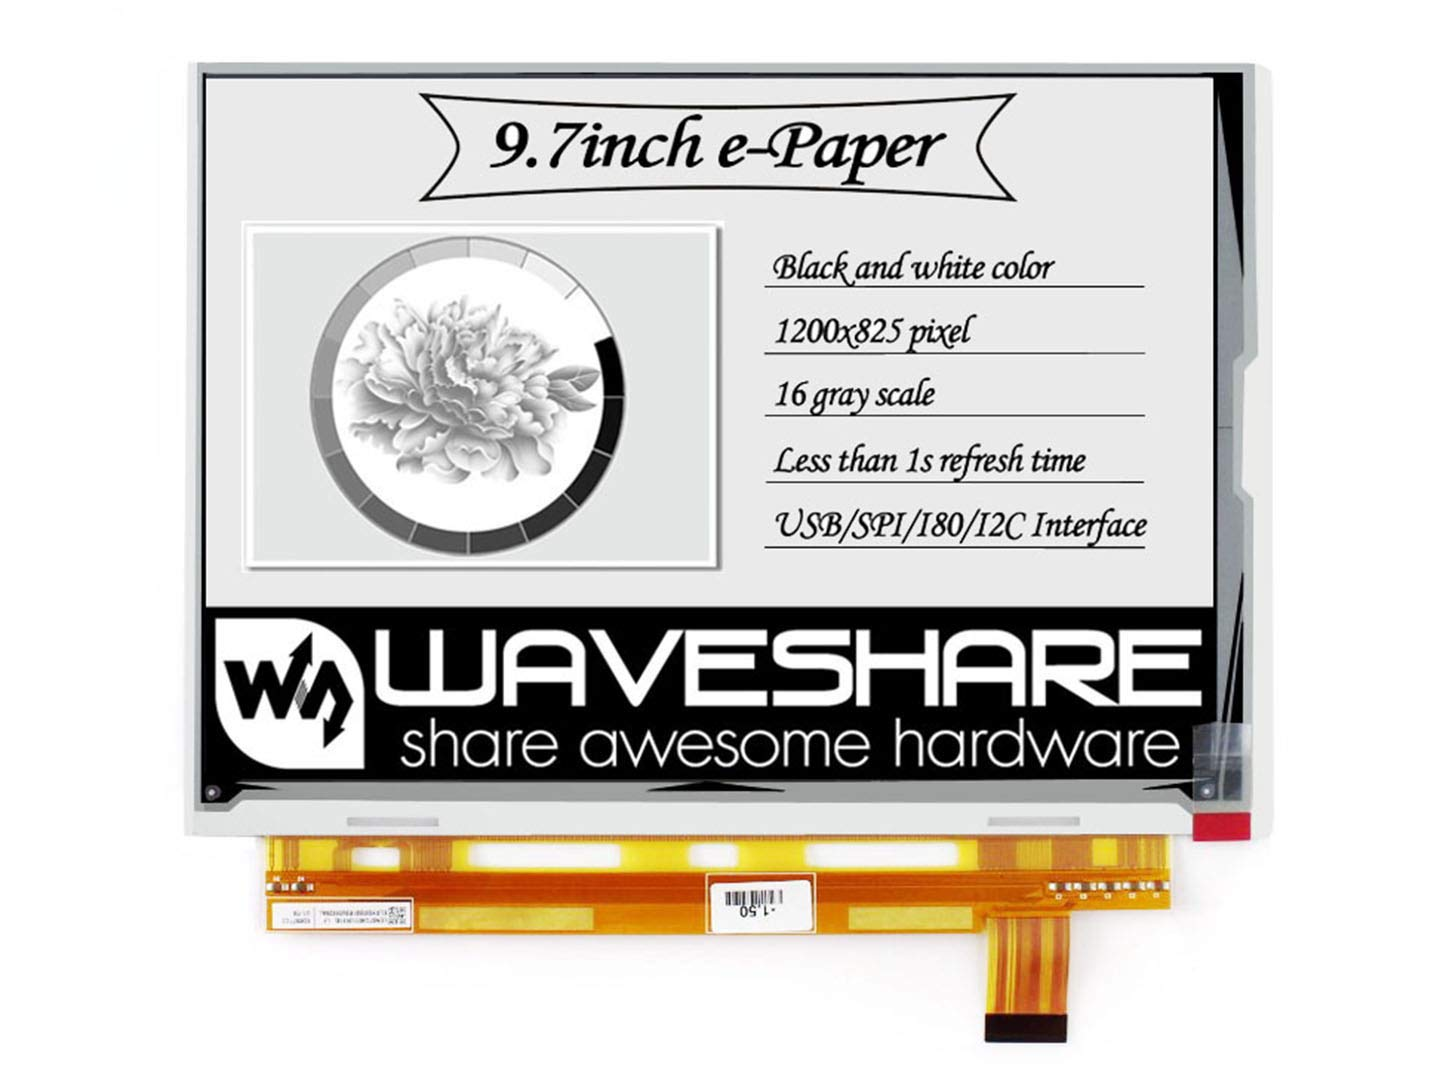
\includegraphics[width=4.5cm]{EpaperDisplay.jpg}}};
	\node[right] at (0,-0.4) {\large EPD};
	
	\fill[white, draw=black] (0,-6) rectangle (6,-10);
	\node at (3, -8) {\large EPD Driver};
		
	%Power Management
	\fill[green!20!white] (9-\ed, \ed) rectangle (26+\ed, -4-\ed);
	\fill[green!20!white] (20-\ed, \ed) rectangle (26+\ed, -10-\ed);
	\node[below, green!40!black] at (11.1,\ed) {\huge Power Management};
	
	
	\fill[white, draw=black] (9,0) rectangle ++(6,-4);
	\node at (12,-2) {\pgftext{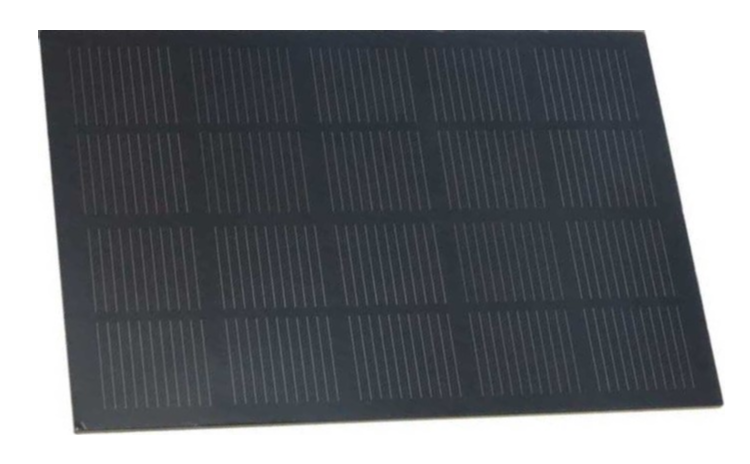
\includegraphics[width=4cm]{solar.png}}};
	\node[right] at (9, -0.4) {\large Solar Cell};
	
	\fill[white, draw=black] (16,0) rectangle ++(3,-3);
	\node at (17.5, -1.5) {\large Super Cap};
	
	\fill[white, draw=black] (20,0) rectangle ++(6,-4);
	\node at (23,-2) {\pgftext{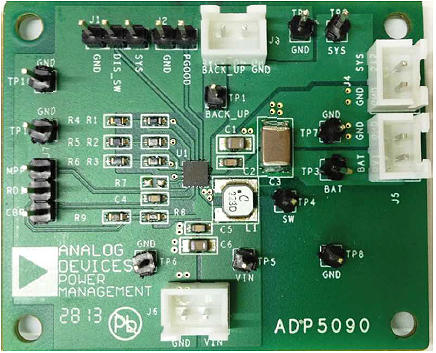
\includegraphics[width=2.5cm]{ADP5090.jpg}}};
	\node[right] at (20, -0.4) {\large ADP5090};
	
	\fill[white, draw=black] (20,-6) rectangle ++(6,-4);
	\node[] at (23, -8) {\large Power Latch};
	%Microcontroller
	\fill[red!20!white] (9-\ed, -6+\ed) rectangle (16.5+\ed, -10-\ed);
	\node[below, red!50!black] at (10.45,-6+\ed) {\huge Microcontroller};
	
	\fill[white, draw=black] (9,-6) rectangle ++(7.5,-4);
	\node[rotate=90] at (12.75,-8) {\pgftext{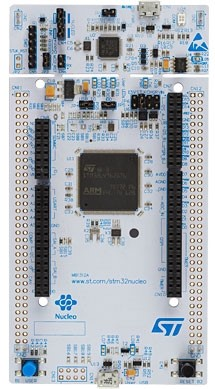
\includegraphics[width=2.2cm]{nucleo.jpg}}};
	\node[right] at (9, -6.4) {\large STM32};
	
	%Communication
	\fill[blue!20!white] (9-\ed, -12+\ed) rectangle (26+\ed, -16-\ed);
	\node[below, blue!50!black] at (10.5,-12+\ed) {\huge Communication};
	
	\fill[white, draw=black] (9,-12) rectangle ++(7.5,-4);
	\node[rotate=90] at (12.75,-14) {\pgftext{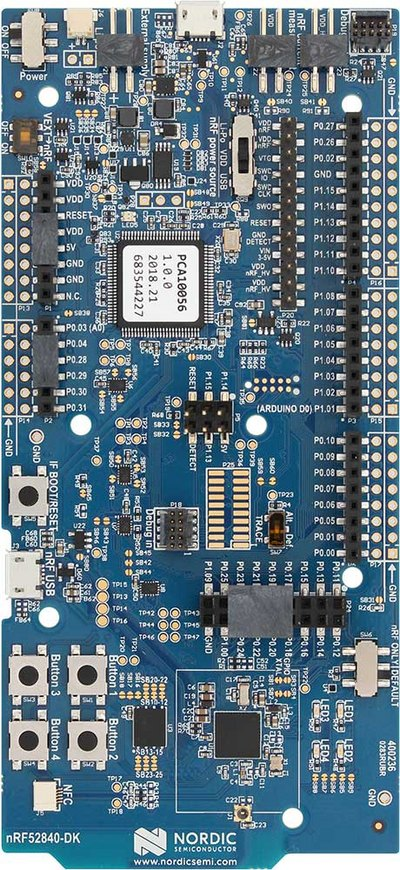
\includegraphics[width=2cm]{nrf52840.jpg}}};
	\node[right] at (9, -12.4) {\Large nRF52840};
	
	\fill[white, draw=black] (20,-12) rectangle ++(6,-4);
	\node[] at (23, -14) {\Large Wakeup Receiver};
				
	%Verbindungen
	\def\len{0.15}
	\def\fs{\footnotesize}
	
	\draw[thick] (0.7,-4) --++(0,\len) node[rotate=90, anchor=west]{\fs EPD};
	\draw[thick] (0.7,-6) --++(0,-\len) node[rotate=90, anchor=east]{\fs EPD};
	\draw[thick] (0.7,-4)--(0.7,-6);
	
	%\draw[thick] (9,-7.5) --++(\len,0) node[right]{\fs SPI};
	\draw[thick] (9,-8.5) --++(\len,0) node[right]{\fs SPI};
	\draw[thick] (9,-9.5) --++(\len,0) node[right]{\fs EPD\_Power};	
	%\draw[thick] (6,-7.5) --++(-\len,0) node[left]{\fs SPI};
	\draw[thick] (6,-8.5) --++(-\len,0) node[left]{\fs SPI};
	\draw[thick] (6,-9.5) --++(-\len,0) node[left]{\fs EPD\_Power};
	%\draw[thick] (9,-7.5)--(6,-7.5);
	\draw[thick] (9,-8.5)--(6,-8.5);
	\draw[thick] (9,-9.5)--(6,-9.5);
	
	\draw[thick] (16.5-0.7,-10) --++(0,\len) node[rotate=90, anchor=west]{\fs UART};
	\draw[thick] (16.5-0.7,-12) --++(0,-\len) node[rotate=90, anchor=east]{\fs UART};
	\draw[thick] (16.5-0.7,-10)--(16.5-0.7,-12);
	
	\draw[thick] (16.5,-6.5) --++(-\len,0) node[left]{\fs SwOFF};
	\draw[thick] (16.5,-7.5) --++(-\len,0) node[left]{\fs $\mu$C\_Power};
	\draw[thick] (20,-6.5) --++(\len,0) node[right]{\fs SwOFF};
	\draw[thick] (20,-7.5) --++(\len,0) node[right]{\fs Power};
	\draw[thick] (16.5,-6.5)--(20,-6.5);
	\draw[thick] (16.5,-7.5)--(20,-7.5);
	
	\draw[thick] (20.7,-10) --++(0,\len) node[rotate=90, anchor=west]{\fs SwON};
	\draw[thick] (20.7,-12) --++(0,-\len) node[rotate=90, anchor=east]{\fs SwON};
	\draw[thick] (20.7,-10)--(20.7,-12);
	
	\draw[thick] (26,-12.5) --++(-\len,0) node[left]{\fs WUR\_Power};
	\draw[thick] (26,-3.5) --++(-\len,0) node[left]{\fs WUR\_Power};
	\draw[thick] (26,-12.5)--(26.6,-12.5)--(26.6,-3.5)--(26,-3.5);
	
	\draw[thick] (23,-4) --++(0,\len) node[rotate=90, anchor=west]{\fs Sys};
	\draw[thick] (23,-6) --++(0,-\len) node[rotate=90, anchor=east]{\fs Sys};
	\draw[thick] (23,-4)--(23,-6);
				
	\draw[thick] (15,-3.5) --++(-\len,0) node[left]{\fs Solar};
	\draw[thick] (20,-3.5) --++(\len,0) node[right]{\fs Solar};
	\draw[thick] (15,-3.5)--(20,-3.5);
	
	\draw[thick] (19,-2.5) --++(-\len,0) node[left]{\fs Cap};
	\draw[thick] (20,-2.5) --++(\len,0) node[right]{\fs Cap};
	\draw[thick] (19,-2.5)--(20,-2.5);
	
	\draw[thick] (16.5,-15.5) --++(-\len,0) node[left]{\fs nRF\_Power};			
	\draw[thick] (16.5,-15.5)--(20-0.6,-15.5)--(20-0.6,-7.5);
	\filldraw (20-0.6,-7.5) circle[radius=1pt];	
				
\end{tikzpicture}
\end{document}